% Template for Cogsci submission with R Markdown

% Stuff changed from original Markdown PLOS Template
\documentclass[10pt, letterpaper]{article}

\usepackage{cogsci}
\usepackage{pslatex}
\usepackage{float}
\usepackage{caption}

% amsmath package, useful for mathematical formulas
\usepackage{amsmath}

% amssymb package, useful for mathematical symbols
\usepackage{amssymb}

% hyperref package, useful for hyperlinks
\usepackage{hyperref}

% graphicx package, useful for including eps and pdf graphics
% include graphics with the command \includegraphics
\usepackage{graphicx}

% Sweave(-like)
\usepackage{fancyvrb}
\DefineVerbatimEnvironment{Sinput}{Verbatim}{fontshape=sl}
\DefineVerbatimEnvironment{Soutput}{Verbatim}{}
\DefineVerbatimEnvironment{Scode}{Verbatim}{fontshape=sl}
\newenvironment{Schunk}{}{}
\DefineVerbatimEnvironment{Code}{Verbatim}{}
\DefineVerbatimEnvironment{CodeInput}{Verbatim}{fontshape=sl}
\DefineVerbatimEnvironment{CodeOutput}{Verbatim}{}
\newenvironment{CodeChunk}{}{}

% cite package, to clean up citations in the main text. Do not remove.
\usepackage{apacite}

% KM added 1/4/18 to allow control of blind submission


\usepackage{color}

% Use doublespacing - comment out for single spacing
%\usepackage{setspace}
%\doublespacing


% % Text layout
% \topmargin 0.0cm
% \oddsidemargin 0.5cm
% \evensidemargin 0.5cm
% \textwidth 16cm
% \textheight 21cm

\title{Parents' Linguistic Alignment Predicts Children's Language Development}


\author{Joseph Denby \and Daniel Yurovsky \\
        \texttt{\{jgdenby, yurovsky\}@uchicago.edu} \\
       Department of Psychology \\ University of Chicago}

\begin{document}

\maketitle

\begin{abstract}
Children quickly gain enormous linguistic knowledge during early
development, in part due to low-level features of their parents' speech.
Some posit that parents contribute to their child's language development
by calibrating their language according to their child's developmental
abilities and needs (Bruner, 1985; Snow, 1972). Here, we investigate
this hypothesis by examining `alignment' at the level of syntax in a
large-scale corpus of parent-child conversations and measuring its
association with language development outcomes. To do so, we employ a
statistical model of alignment to estimate its presence in our dataset
and its impact on language development outcome measures. Our results
corroborate previous findings, showing strong alignment for both parents
and children; in addition, we demonstrate that parental alignment is a
significant predictor of language maturity independent of demographic
features, suggesting that parental tuning has strong ties to a child's
language development.

\textbf{Keywords:}
Language acquisition; computational modeling; cognitive development
\end{abstract}

\hypertarget{introduction}{%
\section{Introduction}\label{introduction}}

Children make vast linguistic strides within their first few years of
life. In light of this some researchers have put forward the linguistic
tuning hypothesis, arguing that parents bolster their child's early
language learning by calibrating the complexity of their speech to the
particular abilities and needs of their children (Montag \& MacDonald,
2015; Snow, 1972; Thiessen, Hill, \& Saffran, 2005). The idea is
intuitive, but it is unclear at what level of language tuning occurs
(Hayes \& Ahrens, 1988; Sokolov, 1993; Spivey \& Dale, 2006) and how
overt it is (Brown \& Hanlon, 1970; Chouinard \& Clark, 2003;
Hirsh-Pasek, Treiman, \& Schneiderman, 1984).

A parallel yet complementary vein of language development research
investigates the presence of low-level cues in parental speech and their
influence on child language learning. From this research, we know that
child-directed speech contains features that facilitate language
learning, and that more exposure tends to result in better outcomes
(Cameron-Faulkner, Lieven, \& Tomasello, 2003; Weisleder \& Fernald,
2013). Related, caregivers from families of high socioeconomic status
(SES) tend to converse more with their children than their lower SES
counterparts, and these increases are associated with improved
development outcomes such as vocabulary size and school performance
(Hoff, 2003; Walker, Greenwood, Hart, \& Carta, 1994). Moreover,
differences in SES-based language development are largely explained by
low-level features of parental child-directed speech such as lexical
diversity and sentence complexity (Hoff-Ginsberg, 1998; Rowe, 2008). So,
given that granular aspects of parental speech can have substantial
effects on a child's language development, it may be that linguistic
tuning occurs at this level in subtle ways, particularly when it comes
to non-content words (i.e., words that are not central to the topic of
discussion.)

This idea of assessing the direct impact of a parent's usage of
non-content word on language development relates to linguistic
alignment, a phenomenon whereby conversational partners tend to align
aspects of their communicative style and content according to various
external influences (Pennebaker, Booth, Boyd, \& Francis, 2015).
Alignment can occur at various levels of language, with some research
(including ours) focusing on the level of syntactic categories (e.g.,
Ireland et al., 2010; Niederhoffer \& Pennebaker, 2016). As an example,
see the exchange between a child and parent presented in Table 1. The
parent's usage of ``across'' directly following their child's usage of
``across'' presents alignment within the syntactic category of
prepositions. Alignment need not involve repetition however; the child's
use of ``I'' following their parent's use of ``I'll'' serves as
alignment within a category as well. Alignment between parents and
children may lend support to the linguistic tuning hypothesis - if
parents align to their children in a way that changes across
development, and that alignment has a concrete impact on a child's
language acquisition, the tuning hypothesis could be vindicated (Bruner,
1985).

Yurovsky, Doyle, \& Frank (2016) investigates linguistic alignment in
CHILDES (MacWhinney, 2000), a natural language corpus of conversations
between parents and children to assess whether tuning occurs at the
level of syntactic categories. They find that syntactic alignment does
occur between both parents and children; moreover, parents align less
over time, suggesting that the relationship their speech shares with
their child's changes as a function of development. These results
present a powerful proof of concept that syntactic alignment exists
between parents and children and changes over time, but it remains
unclear whether alignment bears any sort of concrete, impactful
relationship to language development.

\begin{table}[H]
\centering
\begin{tabular}{ll}
  \hline
  \hline
Parent & I don't know . I'll have to think about it . \\ 
  Child & I was going to do the people across street . \\ 
  Parent & across the street ? \\ 
  Child & yeah . \\ 
   \hline
\end{tabular}
\caption{Excerpt from exchange between 38 month old child and mother in LDP.} 
\end{table}

Here, we extend Yurovsky, Doyle, and Frank's (2016) model by applying it
to the Language Development Project (LDP) (Goldin-Meadow et al., 2014),
a corpus of ecological conversations between parents and their children
over time, collected from a socioeconomically diverse sample of
parent-child dyads. Moreover, we use alignment estimates alongside
demographic information to predict language outcome measures,
strengthening the linguistic tuning hypothesis by concretely showing how
parents' sensitivity to their child's linguistic needs and abilities
covaries with their development.

\hypertarget{model}{%
\section{Model}\label{model}}

The linguistic tuning hypothesis predicts that parents will calibrate
their language in part by assessing their child's needs and abilities.
So, we predict that parents will exhibit high alignment to their young
children, but will reduce their alignment as their children mature. To
test this prediction, we employ an extended version of the Hierarchical
Alignment Model implemented in Yurovsky et al. (2016) which both
estimates the impact of a speaker's use of syntactic categories on their
conversational partner's usage and uses these alignment estimates to
predict language outcome scores.

At base, the model predicts, for each utterance, whether the speaker
will produce a word from a given syntactic category. This prediction is
generated by two factors: the speaker's baseline propensity towards
using that category and the speaker's tendency to align, producing words
from a category just used by their partner. In the model, the primary
computation mimics a standard logistic regression - the production of a
syntactic category within an utterance is treated as a binary outcome
variable impacted by a linear combination of predictor variables (here,
baseline usage and alignment.) The model's hierarchical structure then
allows the estimates of baseline usage and alignment effects to be
pooled across individual speakers and syntactic categories in a way that
ensures statistical robustness.

The model used here then incorporates these alignment and baseline usage
estimates as predictors in a linear regression model of the Pearson
Peabody Vocabulary Test (PPVT) (Dunn \& Dunn, 1997), a widely used
inventory for tracking language development. At this stage, PPVT is
estimated as a linear combination of predictors reflecting alignment and
baseline usage estimate for both parents and children alongside other
features representing demographic variables (e.g., child's gender,
mother's education) and the child's age.

\begin{table}[H]
\centering
\begin{tabular}{ll}
  \hline
category & examples \\ 
  \hline
article & a, alot \\ 
  certain & altogether, must \\ 
  conj & but, or \\ 
  discrep & wanted, hoped \\ 
  excl & whether, not \\ 
  i & i'm, i \\ 
  incl & both, around \\ 
  ipron & thatd, whats \\ 
  negate & needn't, oughtn't \\ 
  preps & at, to \\ 
  quant & series, every \\ 
  tentat & anyhow, most \\ 
  we & we'd, lets \\ 
  you & youd, y'all \\ 
   \hline
\end{tabular}
\caption{LIWC Categories with example words.} 
\end{table}

\hypertarget{model-details}{%
\subsection{Model Details}\label{model-details}}

The structure of the model used here greatly resembles that used in
Yurovsky et al. (2016), in that it operates over utterances represented
as binary vectors, with indices indicating the presence or absence of
each of the 14 LIWC categories (Table 2). The probability of producing
each category in each utterance is computed via two parameters: the
speaker's baseline usage of that syntactic category (\(\eta^{base}\)),
and the change in that speaker's baseline as a function of interacting
with the listener (\(\eta^{align}\)). So, for a given syntactic category
\(c\), for replies to utterances that don't contain \(c\), the
production parameter for that category is computed by applying the
inverse logit function to the appropriate baseline log odds: \[
P(Production_c) = logit^{-1}(\eta^{base}_c)
\] Alternatively, replies to utterances that \emph{do} contain \(c\),
the parameter computation takes into account the sum of the baseline and
alignment log odds: \[
P(Production_c) = logit^{-1}(\eta^{base}_c+\eta^{align}_c)
\]

To accommodate the variance in production across the LIWC categories,
each baseline usage parameter was drawn from an uninformative prior
(\(\eta^{base} \sim Uniform(-5,5)\)); alignment parameters were
regularized towards 0 by way of implementing a conservative prior
(\(\eta^{align} \sim Normal(0,.25)\)).

All parameters were estimated hierarchically, which allows intelligent
pooling of data across participants in the dataset. To start, each
subpopulation (i.e., parents vs.~children) obtained an estimate. Then,
every speaker had an alignment estimate drawn from their appropriate
subpopulation (e.g., if Speaker 22 is a child, their alignment estimate
is drawn from the estimate for children overall.) Category-level
alignment estimates were then drawn for each speaker (e.g., the
alignment estimate for Speaker 22's usage of determiners is drawn from
Speaker 22's alignment estimate.) The order was flipped for baseline
estimates in order to better reflect empirical baseline usages across
syntactic categories; subpopulation estimates produced category-level
estimates, which then produced speaker-level estimates. As in Yurovsky
et al. (2016), we also include parameters that allow baseline and
alignment probabilities to change linearly over time (\(\beta\) and
\(\alpha\) respectively).

Next, we extend the model used in Yurovsky et al. (2016) by using
estimated alignment (i.e., \(\eta\) parameters) to predict PPVT scores,
a measure of vocabulary development (Dunn \& Dunn, 1997). To do so, we
implement a regression model where PPVT scores are modeled as linear
combinations of various predictor variables. These predictor variables
included the child's age, alignment parameter estimates for the child
and their parent, the mother's education, the child's gender, as well as
interaction effects for all variables with age. Error variance for the
model (\(\sigma\)) was also estimated.

The model implemented here then serves two purposes: (1) It extends the
analysis of Yurovsky et al. (2016) to a new dataset, aiming to replicate
previous findings in a more diverse and representative sample, and (2)
It incorporates alignment estimates in a predictive model of early
language outcomes, serving to test the hypothesis that alignment has a
significant relationship with language development, even in the presence
of demographic features. To be specific, we hope to replicate non-zero
estimates for \(\eta\) parameters (demonstrating that alignment between
parents and children exists across datasets), positive \(\beta\) for
children (showing that children increase their baseline usage of
categories over time), and negative \(\alpha\) for parents (showing that
parents decrease their alignment as their children age.) If the PPVT
model estimates for parameters corresponding to the main or interaction
effects of alignment are non-zero in the presence of demographic
variables, we can infer that alignment has an relationship with language
development independent of features like socioeconomic status,
bolstering the linguistic tuning hypothesis.

\hypertarget{analysis}{%
\section{Analysis}\label{analysis}}

\hypertarget{data-and-methodology}{%
\subsection{Data and Methodology}\label{data-and-methodology}}

Conversations between parents and their children were drawn from the
Language Development Project Corpus (Goldin-Meadow et al., 2014).
Participants in the project were videorecorded in their homes for
\(\sim\) 90 minutes every four months starting when the child was
14-months and ending at 58-months. Participants were selected in order
to produce a diverse sample demographically representative of the
broader Chicagoland area.

We selected for analysis all children who were typically developing and
completed at least 10 of the 12 planned recording sessions. Our sample
consisted of 59 target children, 28 of whom were girls, 12 were Black
and 6 were Multiracial. Children were also socio-economically diverse,
as measured by mother's education: 2 mothers had some highschool
education, 7 had a highschool degree, 10 had some college or trade
school, 19 had a highschool degree or GED, 19 had college degrees, and
21 had advanced degrees.

Following Yurovsky et al. (2016), successive utterances from a speaker
within a transcript were concatenated into a single utterance.
Individual utterances were then transformed into binary vectors with
indices indicating the presence or absence of each of the 14 LIWC
categories. This pre-processing turned every transcript into a
speaker-reply format: each utterance within a transcript was both a
reply to the preceding utterance and a message to the next one.

Each transcript was then compressed, yielding 4 numbers for each LIWC
category. For a pair of speakers \emph{A} and \emph{B} in a transcript,
for each LIWC category, we computed the number of utterances from
\emph{A} to \emph{B} containing the category (\(N^{align}\)), the number
of utterances from \emph{A} to \emph{B} not containing the category
(\(N^{base}\)), the number of utterances containing the category
responding to an utterance containing the category (\(C^{align}\)), and
the number of utterances containing the category responding to an
utterance not containing the category (\(C^{base}\)). Aggregating in
this way provided the platform for the model's sampling - for each
transcript, \(C^{base}\) and \(C^{align}\) were drawn from Binomial
distributions parameterized by \(N^{base}\) and \(N^{align}\) chances
respectively, with probabilities computed via the logistic regression
models outlined above.\\
Sampling was performed using Stan, a probabilistic programming language
that implements Hamiltonian Monte Carlo sampling methods (Carpenter et
al., 2017). Posterior distributions for each parameter in the model were
estimated using 500 iterations of Bayesian sampling, generating mean
assessments with appropriate confidence intervals.
\footnote{Data and code available on Github; will be made available at time of unblinding.}

\hypertarget{results}{%
\subsection{Results}\label{results}}

Alignment estimates (\(\eta^{align}\)) for parents and children were
both estimated above zero, corroborating the findings of Yurovsky et al.
(2016) in showing that both groups exhibit alignment (Figure 1). We also
replicate the finding that parents appear to align more to their
children than children align to their parents.

The model estimates developmental baseline changes (\(\beta\)) at
approximately zero for parents, but significantly above zero for
children, replicating previous findings. Alignment is estimated as
having a significantly negative age effect (\(\alpha\)) in this dataset,
replicating an earlier finding that parents tend to exhibit decreased
alignment over their child's development (Figure 3).

\begin{CodeChunk}
\begin{figure}[tb]
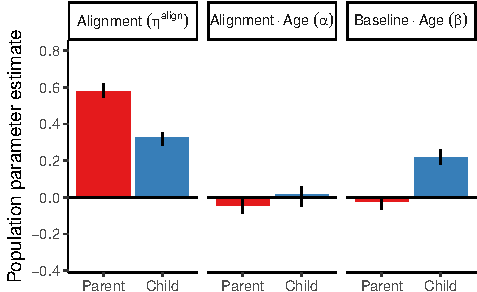
\includegraphics{figs/parameters_plot-1} \caption[Posterior parameter estimates for alignment ($\eta$), developmental change in alignment ($\alpha$), and developmental change in baseline function word production ($\beta$) for both parents and children, as well estimated alignment between parents for a baseline]{Posterior parameter estimates for alignment ($\eta$), developmental change in alignment ($\alpha$), and developmental change in baseline function word production ($\beta$) for both parents and children, as well estimated alignment between parents for a baseline. Bars indicate means, error-bars indicate 95\% highest posterior density intervals generated via Bayesian sampling.}\label{fig:parameters_plot}
\end{figure}
\end{CodeChunk}

The mean estimates for PPVT predictors are presented in Figure 2. PPVT
is positively associated with the age of the child and their being
female. Moreover, female children tend to have a decreased age effect on
PPVT; this means that for female children, the expected increase in PPVT
over time is smaller. Mother's education is negatively associated with
PPVT, but has a slight positive age effect. Alongside these demographic
effects, we see robust alignment effects on PPVT: child and parental
alignment are both associated with increased PPVT, but with decreased
age effects.

\begin{CodeChunk}
\begin{figure}[tb]
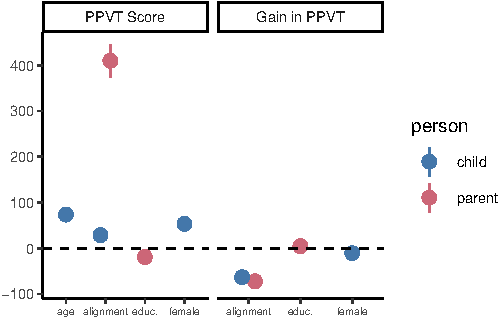
\includegraphics{figs/demopar_plot-1} \caption[Posterior parameter estimates for demographic effects on PPVT scores]{Posterior parameter estimates for demographic effects on PPVT scores. Points indicate means, error-bars indicate 95\% highest posterior density intervals.}\label{fig:demopar_plot}
\end{figure}
\end{CodeChunk}

\begin{CodeChunk}
\begin{figure*}[tb]

{\centering 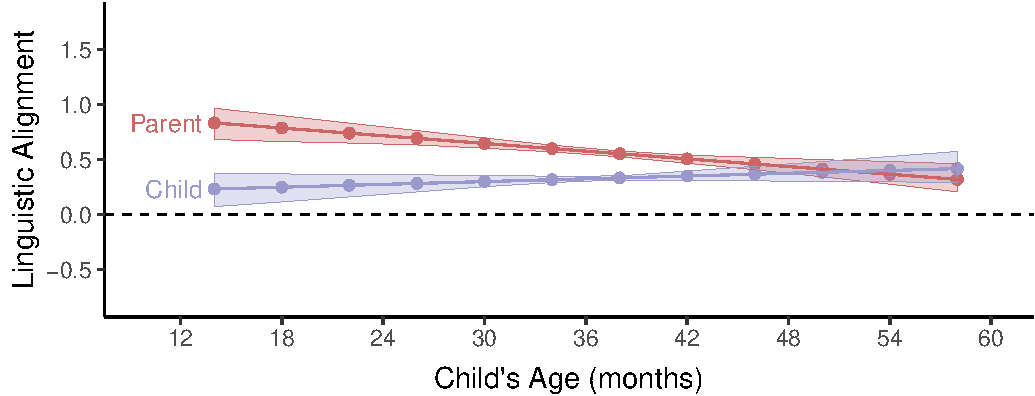
\includegraphics{figs/hpds-1} 

}

\caption[Model-estimated changes in linguistic alignment over development]{Model-estimated changes in linguistic alignment over development. Points indicate the mean of the posterior distribution, shaded regions indicate 68\% highest probability density intervals, equivalent to one standard deviation.}\label{fig:hpds}
\end{figure*}
\end{CodeChunk}

\hypertarget{discussion}{%
\section{Discussion}\label{discussion}}

In an effort to understand and investigate how children rapidly acquire
language, some argue that the language parents produce to their children
is somehow calibrated to the child's particular needs and abilities
(Snow, 1972). While the idea is theoretically compelling, empirical work
has produced mixed results, with strong results in favor of (Chouinard
\& Clark, 2003; Hirsh-Pasek et al., 1984) and against (Brown \& Hanlon,
1970; Hayes \& Ahrens, 1988).

However, much of this prior work investigates tuning as an overt effort
on behalf of parents or tuning with respect to content words, with less
examining the potential role of low-level syntactic influence (Hoff,
2003). Yurovsky et al. (2016) presents just such an examination,
demonstrating using Bayesian hierarchical modeling that parents align to
their children according to their particular language usage at the level
of syntactic categories. This paper extends their model by applying it
to a new socioeconomically diverse sample of families (Goldin-Meadow et
al., 2014) and leveraging the model's alignment estimates to predict
language development outcomes.

The analysis presented here replicates the findings of Yurovsky et al.
(2016), showing strong alignment effects for both parents and their
children, a substantial age effect for baseline useage in children, and
a significant negative effect of age on alignment for parents. Moreover,
we demonstrate that these alignment estimates have substantial power in
predicting language development outcomes, even in the presence of
demographic features such as gender and socioeconomic status. We
corroborate previous findings that female children tend to have higher
PPVT scores that diminish over time (Kaushanskaya, Gross, \& Buac, 2013;
Lange, Euler, \& Zaretsky, 2016). We conflict with other findings that
positively associate child PPVT scores with mother's education (Di
Cesare, Sabates, \& Lewin, 2013; Schady, 2011); this may be due to
idiosyncracies of our dataset, including its limited size.

We show that parental alignment is associated with a relatively large
boost in overall PPVT scores, but with a negative age effect. The
negative age effect may source from a ceiling on PPVT - children with
higher scores may simply have less ground to cover. Nevertheless, these
results are consistent with a concrete effect of parental alignment on
language development, and the linguistic tuning hypothesis more broadly.
A similar story is evident from child alignment estimates: alignment has
a small association with overall PPVT score and an age effect comparable
to parental alignment. Here there may be a confound with childrens'
baseline language production, in that children with lower production
will have lower PPVT and diminished alignment as a result; future work
should assess this interaction to better isolate the effects of
alignment.

Overall, these results show that parental alignment is a robust effect
that appears to have a relationship with childrens' language development
independent of demographic correlates, serving to further the linguistic
tuning hypothesis.

\hypertarget{references}{%
\section{References}\label{references}}

\setlength{\parindent}{-0.1in} 
\setlength{\leftskip}{0.125in}

\noindent

\hypertarget{refs}{}
\leavevmode\hypertarget{ref-Brown:1970wd}{}%
Brown, R. W., \& Hanlon, C. (1970). Derivational Complexity and Order of
Acquisition in Child Speech. In J. Hayes (Ed.), \emph{Cognition and the
development of language} (pp. 11--53). New York.

\leavevmode\hypertarget{ref-Bruner:1985if}{}%
Bruner, J. (1985). Child's Talk: Learning to Use Language. \emph{Child
Language Teaching and Therapy}, \emph{1}(1), 111--114.

\leavevmode\hypertarget{ref-CameronFaulkner:2003ge}{}%
Cameron-Faulkner, T., Lieven, E., \& Tomasello, M. (2003). A
construction based analysis of child directed speech. \emph{Cognitive
Science}, \emph{27}(6), 843--873.

\leavevmode\hypertarget{ref-Carpenter:2017ke}{}%
Carpenter, B., Gelman, A., Hoffman, M. D., Lee, D., Goodrich, B.,
Betancourt, M., \ldots{} Riddell, A. (2017). Stan : A Probabilistic
Programming Language. \emph{Journal of Statistical Software},
\emph{76}(1).

\leavevmode\hypertarget{ref-Chouinard:2003kq}{}%
Chouinard, M. M., \& Clark, E. V. (2003). Adult reformulations of child
errors as negative evidence. \emph{Journal of Child Language},
\emph{30}(3), 637--669.

\leavevmode\hypertarget{ref-DiCesare:2013ip}{}%
Di Cesare, M., Sabates, R., \& Lewin, K. M. (2013). A double prevention:
how maternal education can affect maternal mental health, child health
and child cognitive development. \emph{Longitudinal and Life Course
Studies}, \emph{4}.

\leavevmode\hypertarget{ref-PeabodyPictureVoca:im}{}%
Dunn, L. M., \& Dunn, L. M. (1997). Peabody Picture Vocabulary
Test--Third Edition. \emph{PsycTESTS Dataset}.

\leavevmode\hypertarget{ref-GoldinMeadow:2014hr}{}%
Goldin-Meadow, S., Levine, S. C., Hedges, L. V., Huttenlocher, J.,
Raudenbush, S. W., \& Small, S. L. (2014). New evidence about language
and cognitive development based on a longitudinal study: Hypotheses for
intervention. \emph{American Psychologist}, \emph{69}(6), 588--599.

\leavevmode\hypertarget{ref-Hayes:1988ue}{}%
Hayes, D. P., \& Ahrens, M. G. (1988). Vocabulary simplification for
children: a special case of 'motherese'? \emph{Journal of Child
Language}, \emph{15}(2), 395--410.

\leavevmode\hypertarget{ref-HirshPasek:1984bd}{}%
Hirsh-Pasek, K., Treiman, R., \& Schneiderman, M. (1984). Brown \&
Hanlon revisited: mothers' sensitivity to ungrammatical forms.
\emph{Journal of Child Language}, \emph{11}(01), 81--88.

\leavevmode\hypertarget{ref-Hoff:2003kx}{}%
Hoff, E. (2003). The specificity of environmental influence:
Socioeconomic status affects early vocabulary development via maternal
speech. \emph{Child Development}, \emph{74}(5), 1368--1378.

\leavevmode\hypertarget{ref-HoffGinsberg:2008up}{}%
Hoff-Ginsberg, E. (1998). The relation of birth order and socioeconomic
status to children's language experience and language development.
\emph{Applied Psycholinguistics}, \emph{19}, 603--629.

\leavevmode\hypertarget{ref-Ireland:2010gl}{}%
Ireland, M. E., Slatcher, R. B., Eastwick, P. W., Scissors, L. E.,
Finkel, E. J., \& Pennebaker, J. W. (2010). Language Style Matching
Predicts Relationship Initiation and Stability. \emph{Psychological
Science}, \emph{22}(1), 39--44.

\leavevmode\hypertarget{ref-Kaushanskaya:2013gi}{}%
Kaushanskaya, M., Gross, M., \& Buac, M. (2013). Gender differences in
child word learning. \emph{Learning and Individual Differences},
\emph{27}, 82--89.

\leavevmode\hypertarget{ref-Lange:2016gv}{}%
Lange, B. P., Euler, H. A., \& Zaretsky, E. (2016). Sex differences in
language competence of 3- to 6-year-old children. \emph{Applied
Psycholinguistics}, \emph{37}(06), 1417--1438.

\leavevmode\hypertarget{ref-MacWhinney:2000jx}{}%
MacWhinney, B. (2000). The CHILDES Project. \emph{Computational
Linguistics}, \emph{26}(4), 657--657.

\leavevmode\hypertarget{ref-Montag:2015iy}{}%
Montag, J. L., \& MacDonald, M. C. (2015). Text exposure predicts spoken
production of complex sentences in 8- and 12-year-old children and
adults. \emph{Journal of Experimental Psychology: General},
\emph{144}(2), 447--468.

\leavevmode\hypertarget{ref-Niederhoffer:2016co}{}%
Niederhoffer, K. G., \& Pennebaker, J. W. (2016). Linguistic Style
Matching in Social Interaction. \emph{Journal of Language and Social
Psychology}, \emph{21}(4), 337--360.

\leavevmode\hypertarget{ref-Pennebaker:kqtgxul0}{}%
Pennebaker, J. W., Booth, R. J., Boyd, R. L., \& Francis, M. E. (2015).
Linguistic inquiry and word count: LIWC2015. Austin, TX: Pennebaker
Conglomerates.

\leavevmode\hypertarget{ref-ROWE:2008go}{}%
Rowe, M. L. (2008). Child-directed speech: relation to socioeconomic
status, knowledge of child development and child vocabulary skill.
\emph{Journal of Child Language}, \emph{35}(01), 185--205.

\leavevmode\hypertarget{ref-Schady:2011bb}{}%
Schady, N. (2011). Parents' education, mothers' vocabulary, and
cognitive development in early childhood: longitudinal evidence from
Ecuador. \emph{American Journal of Public Health}, \emph{101}(12),
2299--2307.

\leavevmode\hypertarget{ref-Snow:2018wf}{}%
Snow, C. E. (1972). Mothers' Speech to Children Learning Language.
\emph{Child Development}, \emph{43}(2), 549--565.

\leavevmode\hypertarget{ref-Sokolov:1993cr}{}%
Sokolov, J. L. (1993). A local contingency analysis of the fine-tuning
hypothesis. \emph{Developmental Psychology}, \emph{29}(6), 1008--1023.

\leavevmode\hypertarget{ref-Spivey:2006fa}{}%
Spivey, M. J., \& Dale, R. (2006). Continuous Dynamics in Real-Time
Cognition. \emph{Current Directions in Psychological Science},
\emph{15}(5), 207--211.

\leavevmode\hypertarget{ref-Thiessen:2005tx}{}%
Thiessen, E. D., Hill, E. A., \& Saffran, J. R. (2005). Infant-Directed
Speech Facilitates Word Segmentation. \emph{Infancy}, \emph{7}(1),
53--71.

\leavevmode\hypertarget{ref-Anonymous:GIFaG1Qd}{}%
Walker, D., Greenwood, C., Hart, B., \& Carta, J. (1994). Prediction of
School Outcomes Based on Early Language Production and Socioeconomic
Factors. \emph{Children and Poverty}, \emph{65}(2), 606--621.

\leavevmode\hypertarget{ref-Weisleder:2013ht}{}%
Weisleder, A., \& Fernald, A. (2013). Talking to Children Matters.
\emph{Psychological Science}, \emph{24}(11), 2143--2152.

\leavevmode\hypertarget{ref-Anonymous:r2JoRscQ}{}%
Yurovsky, D., Doyle, G., \& Frank, M. C. (2016). Linguistic input is
tuned to children's developmental level. In \emph{Proceedings of the
annual meeting of the cognitive science society} (pp. 2093--2098).

\bibliographystyle{apacite}


\end{document}
